\chapter{Filtered Colimits, Coends, and Kan Extensions}

\section{Filtered Categories and Limits}

Outside of category theory, the most common types of limits that are taken 
in areas such as algebraic geometry and topology are inverse and directed limits. 
These are limits which are taken over thin categories (or preorders) which have at 
most one morphism between any two morphisms. 

As we shall see, limits over thin categories do not possess the nice 
properties that limits taken over \emph{filtered} categories have, which we will 
see is the categorification 
of the notion of a \emph{directed set}. We will motivate our desire to 
work with filtered categories instead of just thin categories
by observing an analogous motivation to work with 
directed sets instead of $\mathbb{N}$ in sequences within topology. 
The picture in mind should be:

\begin{center}
    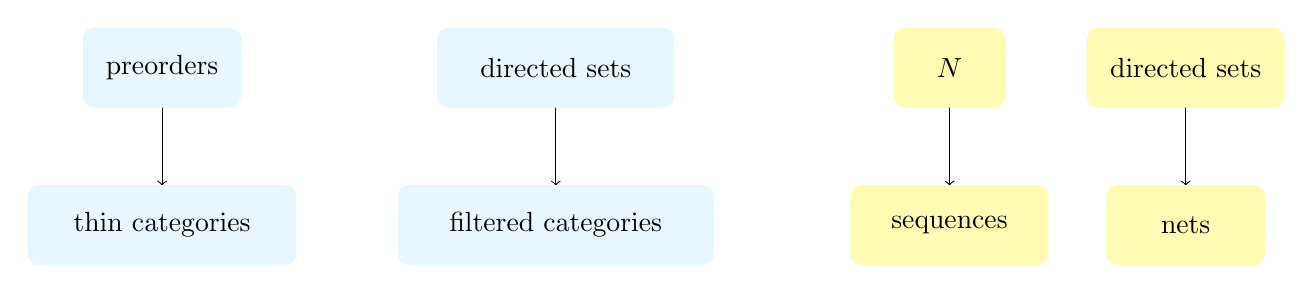
\begin{tikzpicture}
        \begin{scope}[xshift = -3cm]
            \draw[->] (0,-0.5)--(0, -1.5);
            \draw[->] (5,-0.5)--(5, -1.5);
            \filldraw[rounded corners, ProcessBlue!10]
            (-1,-0.5) rectangle (1, 0.5);
            \node at (0,0) {preorders};
    
            \begin{scope}[xshift = 5cm]
                \filldraw[rounded corners, ProcessBlue!10]
                (-1.5,-0.5) rectangle (1.5, 0.5);
                \node at (0,0) {directed sets};
            \end{scope}
    
            \begin{scope}[yshift = -2cm]
                \filldraw[rounded corners, ProcessBlue!10]
                (-1.7,-0.5) rectangle (1.7, 0.5);
                \node at (0,0) {thin categories};
            \end{scope}
    
            \begin{scope}[xshift = 5cm, yshift=-2cm]
                \filldraw[rounded corners, ProcessBlue!10]
                (-2,-0.5) rectangle (2, 0.5);
                \node at (0,0) {filtered categories};
            \end{scope}
        \end{scope}

        \begin{scope}[xshift = 7cm]
            \draw[->] (0,-0.5)--(0, -1.5);
            \draw[->] (3,-0.5)--(3, -1.5);
            \filldraw[rounded corners, yellow!30]
            (-0.7,-0.5) rectangle (0.7, 0.5);
            \node at (0,0) {$\mathbb{N}$};
    
            \begin{scope}[xshift = 3cm]
                \filldraw[rounded corners, yellow!30]
                (-1.25,-0.5) rectangle (1.25, 0.5);
                \node at (0,0) {directed sets};
            \end{scope}
    
            \begin{scope}[yshift = -2cm]
                \filldraw[rounded corners, yellow!30]
                (-1.25,-0.5) rectangle (1.25, 0.5);
                \node at (0,0) {sequences};
            \end{scope}
    
            \begin{scope}[xshift = 3cm, yshift=-2cm]
                \filldraw[rounded corners, yellow!30]
                (-1,-0.5) rectangle (1, 0.5);
                \node at (0,0) {nets};
            \end{scope}
        \end{scope}
    \end{tikzpicture}

    \emph{On the left, we see that thin and filtered categories are the categorification of 
    concepts which we will use to take limits over. On the right, we have topology concepts 
    of sequences and nets, which are limits taken over different sets. }
\end{center}

Let $X$ be a topological space. Recall that a sequence $\{a_n\}_{n=1}^{\infty}$ in $X$ is a function 
$a: \mathbb{N}\to X$ such that $a(n) = a_n$. We say the sequence converges to a point 
$x \in X$ if for every open set $U$ of $x$ there exists a
$N \in \mathbb{N}$ such that $\{a_N, a_{N+1}, \dots, \} \subset U$. 

Some of the first topological spaces that people worked with were metric spaces $(X, d)$, 
and the properties of these spaces were worked out over time. People eventually figured out 
that 
\begin{itemize}
    \item A subset $F \subset X$ is closed if and only if $F$ contains 
    the limits of every sequence in $F$.
    \item A subset $U \subset X$ is open if and only if $U$ contains 
    does not contain the limit of any sequence in $X - U$. 
\end{itemize}
This is a wonderful result! However, it does not generalize to arbitrary topological 
spaces. There are weird counterexamples that we will not get into (cite An Introduction 
to Topology and Homotopy Theory by Sierdaski).

What this means is that sequences over a plain preorder (i.e., $\mathbb{N}$) are great, and they 
have nice 
properties, but they lack the ability to extend their nice properties to arbitrary 
topological spaces. We need more if we want it to work over arbitrary spaces. 

This is where a directed set comes in. 
\begin{definition}
    A \textbf{directed set} $D$ is a set equipped with a binary relation $\le$ such that 
    for all $a, b, c \in D$,
    \begin{description}
        \item[\textbf{1.}] $a \le a$ (Reflexive).
        \item[\textbf{2.}] if $a \le b$ and $b \le c$, then $a \le c$ (Transitive)
        \item[\textbf{3.}] For all $a,b \in D$, there exists a $c \in C$ such that $a \le c$ \textbf{and} $b \le c$ (Directed).
    \end{description}
    The first two properties describe a preorder; only the last condition is new to us. 
    To summarize, the ``directed'' axiom grants us an upper bounded in $D$ for any finite 
    set of elements of $D$.  

    Let $D$ be a directed set. Define a \textbf{net}, or \textbf{Moore-Smtih Sequence}, 
    to be a function $\lambda: D \to X$. We say a net $\lambda$ converges to a point $x \in X$
    if for every open set $U$ containing $x$, there exists a $d \in D$ such that 
    $\{\lambda(c) \mid c \ge d\} \subset U$. 
\end{definition}

Directed sets are then enough to give us the following theorem:
\begin{theorem}
    Let $X$ be a topological space.
    \begin{itemize}
        \item A subset $F \subset X$ is closed if and only if every convergent 
        net $\lambda: D \to X$ has a limit in $F$
        \item A subset $U \subset X$ is open if and only if every convergent net 
        $\lambda: D \to X - U$ does not have a limit in $U$.
    \end{itemize}
\end{theorem}

Hence we see that limits taken over preorders have substantial benefits than when 
they are simply taken over $\mathbb{N}$. Similarly, what we will see is that 
limits taken over filtered categories enjoy much better properties than limits 
simply taken over preorders. First, we introduce filtered categories.

\begin{definition}
    We say that a category $J$ is \textbf{filtered} if 
    \begin{itemize}
        \item[\textbf{1.}] For any pair of objects $j, j'$, 
        there exists an object $k$ and morphism $u:j \to k$ and $v: j' \to k$. 
        \item[\textbf{2.}] For any pair of parallel morphism $u, v: i \to j$, 
        there exists an object $k$ and a morphism $w: j \to k$ such that the diagram below 
        commutes. 
    \end{itemize}    
    We do not say the empty category is filtered; this should be obvious, but 
    it also needs to be said.

    \begin{center}
        \begin{tikzpicture}
            \filldraw[rounded corners, Yellow!30]
            (-2.25, -1.5) rectangle (2.25, 1.5);
            \node at (0,0){
                \begin{tikzcd}[column sep = 1.4cm, row sep = 0.3cm]
                    j 
                    \arrow[dr, "u"]& 
                    \\
                    &
                    k
                    \\
                    j' \arrow[ur, swap, "v"]
                \end{tikzcd}
            };
            \begin{scope}[xshift = 7cm]
                \filldraw[rounded corners, Yellow!30]
                (-2.25, -1.5) rectangle (2.25, 1.5);
                \node at (0,0){
                    \begin{tikzcd}[column sep = 1.4cm, row sep = 0.5cm]
                        &
                        j
                        \arrow[dr, dashed, "w"]
                        &
                        \\
                        i \arrow[ur, "u"] 
                        \arrow[dr, dashed, swap, "v"]
                        & 
                        & 
                        k
                        \\
                        &
                        j 
                        \arrow[ur, dashed, swap, "w"]
                        &
                    \end{tikzcd}
                };
            \end{scope}
        \end{tikzpicture}

        \emph{Conditions (1) and (2) illustrated.}
    \end{center}
    
    
\end{definition}

\begin{example}
    Let $J$ be a thin category. What does it take for $J$ to be filtered? 
    Well, in a thin category, there is never 
    any pair of distinct morphisms. Hence condition (2) is trivial. Therefore, 
    for $J$ to be filtered, we simply need to satisfy (1). But in the language 
    of thin categories, condition (1) can be read as ``for any $j, j \in J$, 
    there exists a $k$ such that $j, j' \le k$''. Such a condition holds 
    if and only if
    \begin{center}
        every finite subset $S \subset J$ has an upper bound \emph{in} $J$.
    \end{center}
    Thus, a thin category $J$ needs to have the above property in order to 
    be a filtered category.

    An example of this concerns the category $\textbf{Open}(X)$, where 
    $X$ is a topological space. The objects are open sets, while morphisms are 
    inclusions. The maximal element $X \in \textbf{Open}(X)$
    always exists, and hence makes this thin category filtered.
\end{example}